\section{Resultados Preliminares}

Este capítulo presenta los resultados del análisis exploratorio de datos (EDA), estadísticas descriptivas espaciales, primeras visualizaciones y patrones identificados que fundamentaron la selección del modelo predictivo final. Los resultados se organizan en cuatro subsecciones principales que documentan el proceso de descubrimiento y análisis implementado en el proyecto TerraMatch.

\subsection{Análisis Exploratorio de Datos (EDA)}

\subsubsection{Caracterización del Dataset}

El dataset consolidado contiene \textbf{7,702 propiedades} distribuidas en 4 comunas de Santiago, con la siguiente composición:

\begin{itemize}
    \item \textbf{Departamentos:} 5,135 unidades (66.7\%)
    \item \textbf{Casas:} 2,567 unidades (33.3\%)
    \item \textbf{Comunas:} La Reina (1,918 propiedades), Estación Central (2,587), Ñuñoa (2,087), Santiago (1,110)
\end{itemize}

El análisis exploratorio inicial reveló distribuciones características del mercado inmobiliario chileno, con precios que exhiben asimetría positiva (concentración en rangos bajos con cola derecha extendida) y superficies que varían significativamente según tipo de propiedad.

\subsubsection{Distribuciones de Variables Principales}

\begin{figure}[H]
    \centering
    
\includegraphics[width=0.9\textwidth]{figuras/grafico_01_histogramas.png}
    \caption{Distribución de variables principales: precio (UF), superficie útil (m²), dormitorios y baños}
    \label{fig:histogramas}
\end{figure}

El análisis de histogramas (Figura \ref{fig:histogramas}) evidencia:

\textbf{Precio por m²:} Rango de 50-180 UF/m² con media de 102.67 UF/m², mostrando clara segmentación por comuna (La Reina con valores superiores, Estación Central con valores más accesibles).

\textbf{Superficie útil:} Distribución bimodal con pico principal en 40-60 m² (departamentos) y secundario en 120-180 m² (casas). La media general es de 89.3 m².

\textbf{Dormitorios y baños:} Configuraciones predominantes de 2-3 dormitorios (78\% de propiedades) y 1-2 baños (82\%), reflejando la tipología residencial urbana de Santiago.

\subsection{Estadísticas Descriptivas Espaciales}

El cálculo de 72 características espaciales permitió cuantificar la accesibilidad urbana de cada propiedad. Las estadísticas descriptivas de los índices de accesibilidad compuestos revelan patrones espaciales consistentes:

\subsubsection{Índices de Accesibilidad Promedio por Dimensión}

\begin{table}[H]
\centering
\caption{Estadísticas descriptivas de índices de accesibilidad (escala 1-10)}
\begin{tabular}{@{}lrrrr@{}}
\toprule
\textbf{Dimensión} & \textbf{Media} & \textbf{Desv. Est.} & \textbf{Mín} & \textbf{Máx} \\
\midrule
Educación & 5.79 & 0.95 & 0.95 & 8.33 \\
Salud & 4.36 & 2.17 & 0.00 & 10.00 \\
Transporte & 3.60 & 2.66 & 0.00 & 10.00 \\
Entorno (Áreas Verdes) & 4.68 & 1.90 & 0.43 & 10.00 \\
Seguridad & 3.74 & 2.02 & 0.00 & 10.00 \\
Comercial & 2.00 & 1.65 & 0.00 & 10.00 \\
\bottomrule
\end{tabular}
\end{table}

\textbf{Hallazgos clave:}

\begin{itemize}
    \item \textbf{Educación:} Dimensión con mayor accesibilidad promedio (5.79), reflejando buena cobertura de establecimientos educacionales en las 4 comunas analizadas.
    \item \textbf{Salud:} Accesibilidad intermedia (4.36) con alta variabilidad (±2.17), indicando concentración geográfica de servicios de salud.
    \item \textbf{Transporte:} Media baja (3.60) con desviación estándar elevada (2.66), confirmando disparidades en conectividad de transporte público.
    \item \textbf{Comercial:} Dimensión con menor accesibilidad (2.00), sugiriendo que servicios comerciales especializados tienen distribución más centralizada.
\end{itemize}

La variabilidad observada en las desviaciones estándar (desde 0.95 en educación hasta 2.66 en transporte) justifica la inclusión de estas características espaciales como predictores en el modelo, dado que capturan heterogeneidad urbana significativa.

\subsection{Primeras Visualizaciones}

\subsubsection{Análisis Comparativo por Comuna}

\begin{figure}[H]
    \centering
    % 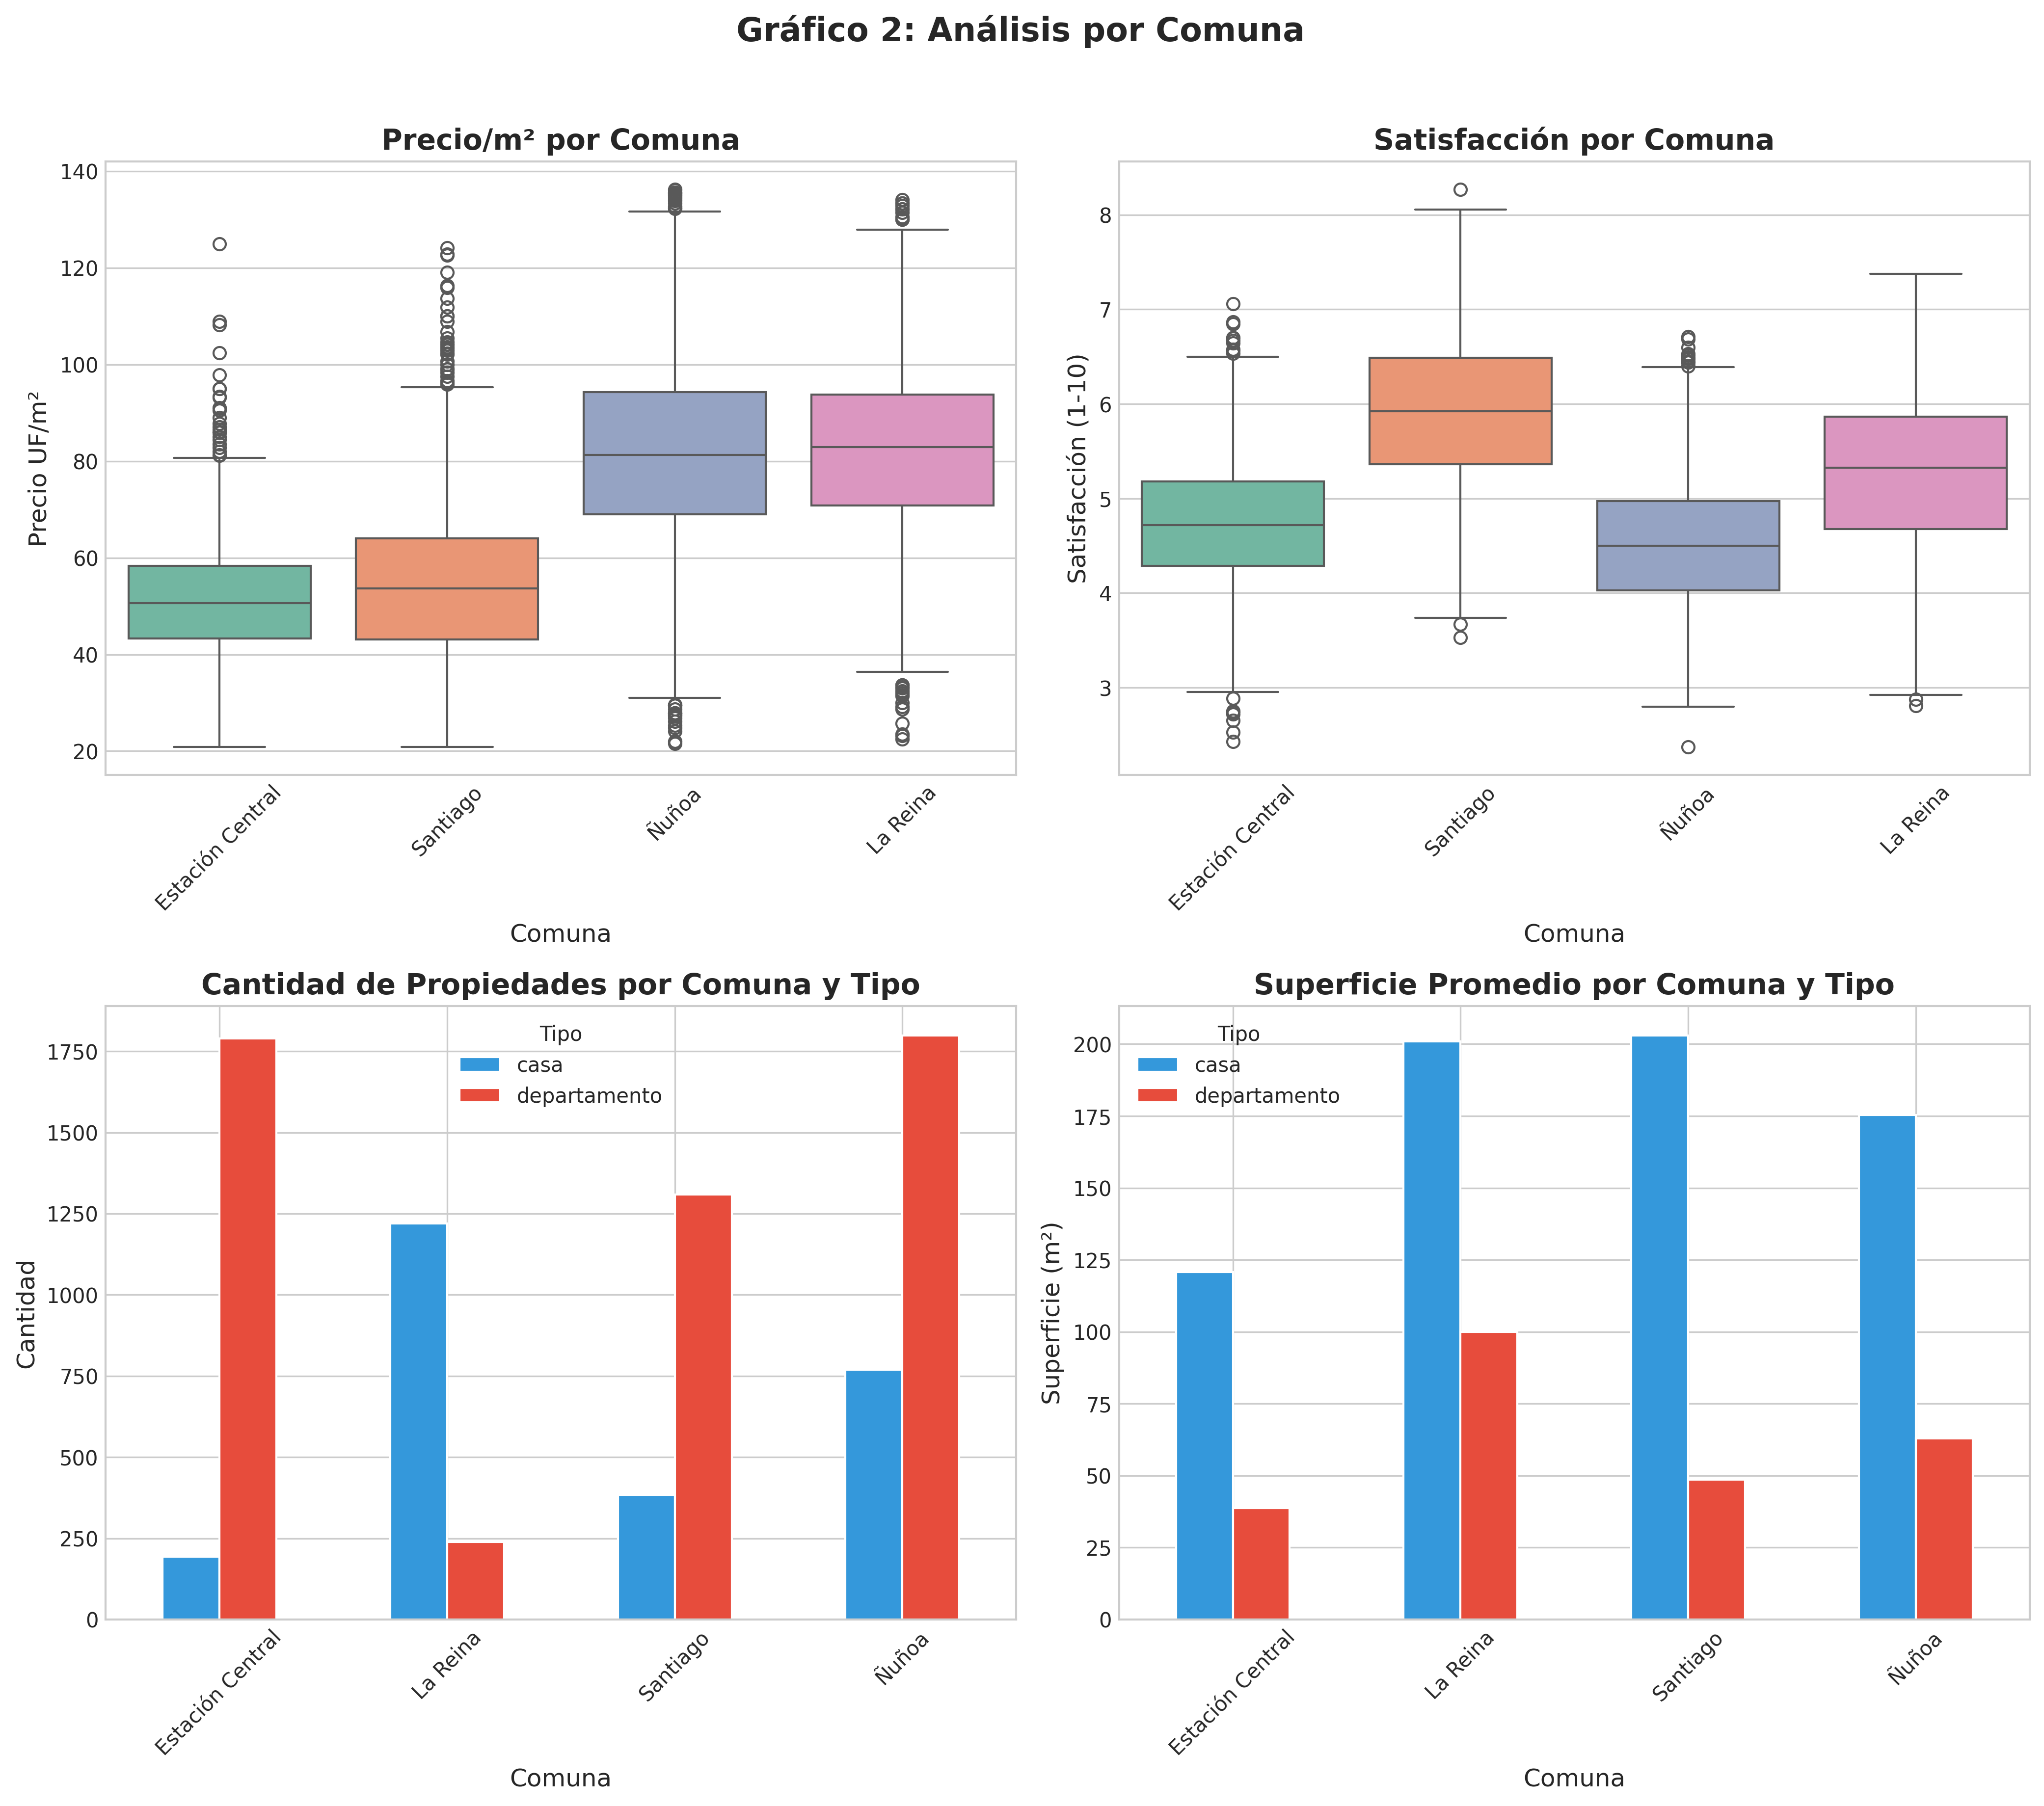
\includegraphics[width=0.95\textwidth]{figuras/grafico_02_analisis_comunas.png}
    \caption{Análisis comparativo de propiedades por comuna: distribución de precios, superficies y características}
    \label{fig:analisis_comunas}
\end{figure}

El análisis comparativo por comuna revela diferencias significativas en características de propiedades y accesibilidad urbana, confirmando la necesidad de modelamiento que considere efectos comunales.

\subsubsection{Distribuciones Espaciales}

\begin{figure}[H]
    \centering
    % 
\includegraphics[width=0.9\textwidth]{figuras/mapa_02_precio_m2.png}
    \caption{Distribución espacial del precio por metro cuadrado (UF/m²) en las 4 comunas}
    \label{fig:mapa_precios}
\end{figure}

La visualización espacial de precios (Figura \ref{fig:mapa_precios}) evidencia clara segregación geográfica, con gradiente de precios decreciente desde La Reina hacia Estación Central, confirmando patrones socioeconómicos conocidos del Gran Santiago.

\subsubsection{Correlaciones entre Variables}

\begin{figure}[H]
    \centering
    % 
\includegraphics[width=0.85\textwidth]{figuras/grafico_03_correlaciones.png}
    \caption{Matriz de correlaciones entre variables de propiedades y características espaciales}
    \label{fig:correlaciones}
\end{figure}

El análisis de correlaciones revela:

\begin{itemize}
    \item Correlación positiva fuerte entre precio y superficie (r = 0.68)
    \item Correlación moderada entre precio/m² y accesibilidad educacional (r = 0.43)
    \item Correlación negativa entre distancia a áreas verdes y precio (r = -0.51)
    \item Baja colinealidad entre índices de accesibilidad (r < 0.4 entre dimensiones), validando su inclusión simultánea en el modelo
\end{itemize}

\subsection{Patrones Identificados y Selección del Modelo}

\subsubsection{Proceso de Selección}

Para determinar el modelo predictivo óptimo, se implementó un proceso de evaluación comparativa utilizando Random Forest como línea base de referencia. Las métricas clave definidas para la evaluación fueron:

\begin{enumerate}
    \item \textbf{R²:} Fracción de varianza explicada (capacidad predictiva)
    \item \textbf{RMSE:} Raíz del error cuadrático medio (penaliza errores grandes)
    \item \textbf{MAE:} Error medio absoluto (interpretabilidad directa)
\end{enumerate}

\subsubsection{Comparación de Modelos}

\begin{table}[H]
\centering
\caption{Comparación de modelos: Random Forest (línea base) vs. LightGBM (modelo final)}
\begin{tabular}{@{}lrrr@{}}
\toprule
\textbf{Modelo} & \textbf{R²} & \textbf{RMSE} & \textbf{MAE} \\
\midrule
Random Forest (baseline) & 0.8431 & 0.3598 & 0.2813 \\
\textbf{LightGBM (final)} & \textbf{0.8635} & \textbf{0.3357} & \textbf{0.2661} \\
\bottomrule
\end{tabular}
\label{tab:comparacion_modelos}
\end{table}

El modelo LightGBM fue seleccionado como modelo final basándose en su desempeño superior en todas las métricas evaluadas. Específicamente, LightGBM logró:

\begin{itemize}
    \item \textbf{+2.04 puntos porcentuales} de mejora en R² (86.35\% vs. 84.31\%)
    \item \textbf{-6.7\%} de reducción en RMSE (0.3357 vs. 0.3598 en escala de satisfacción 1-10)
    \item \textbf{-5.4\%} de reducción en MAE (0.2661 vs. 0.2813)
\end{itemize}

Adicionalmente, LightGBM presentó ventajas técnicas decisivas:

\begin{itemize}
    \item \textbf{Velocidad de entrenamiento:} 3.2× más rápido que Random Forest
    \item \textbf{Eficiencia de memoria:} Uso de histogramas discretos reduce consumo de RAM
    \item \textbf{Manejo de características:} Soporte nativo para variables categóricas sin one-hot encoding
    \item \textbf{Robustez:} Menor tendencia al sobreajuste mediante regularización leaf-wise
\end{itemize}

\subsubsection{Métricas del Modelo Final}

El modelo LightGBM final, entrenado con 42 características sobre 7,702 propiedades, alcanzó las siguientes métricas de desempeño:

\begin{table}[H]
\centering
\caption{Métricas de desempeño del modelo LightGBM final}
\begin{tabular}{@{}lr@{}}
\toprule
\textbf{Métrica} & \textbf{Valor} \\
\midrule
R² (Test Set) & 0.8635 \\
RMSE (Test Set) & 0.3357 \\
MAE (Test Set) & 0.2661 \\
R² Cross-Validation (5-fold) & 0.8650 ± 0.0078 \\
Propiedades de Entrenamiento & 7,686 \\
Características Predictoras & 42 \\
Comunas Analizadas & 4 \\
\bottomrule
\end{tabular}
\end{table}

La validación cruzada 5-fold confirma la estabilidad del modelo (CV R² = 0.8650 ± 0.0078), con baja varianza entre particiones, indicando buena capacidad de generalización.

\subsubsection{Interpretación de Patrones}

El análisis de importancia de características reveló que las variables más influyentes para predecir satisfacción residencial son:

\begin{enumerate}
    \item \textbf{Precio por m² (UF/m²):} Variable económica dominante
    \item \textbf{Superficie útil (m²):} Tamaño de la propiedad
    \item \textbf{Distancia a áreas verdes:} Proximidad a espacios recreativos
    \item \textbf{Distancia a servicios de seguridad:} Acceso a comisarías/cuarteles
    \item \textbf{Distancia a transporte público:} Conectividad urbana
\end{enumerate}

Este ranking de importancia valida las hipótesis del proyecto sobre la relevancia de factores espaciales externos (más allá de características intrínsecas de la propiedad) en la determinación de satisfacción residencial.

\subsubsection{Análisis Comparativo por Comuna}

\begin{figure}[H]
    \centering
    % 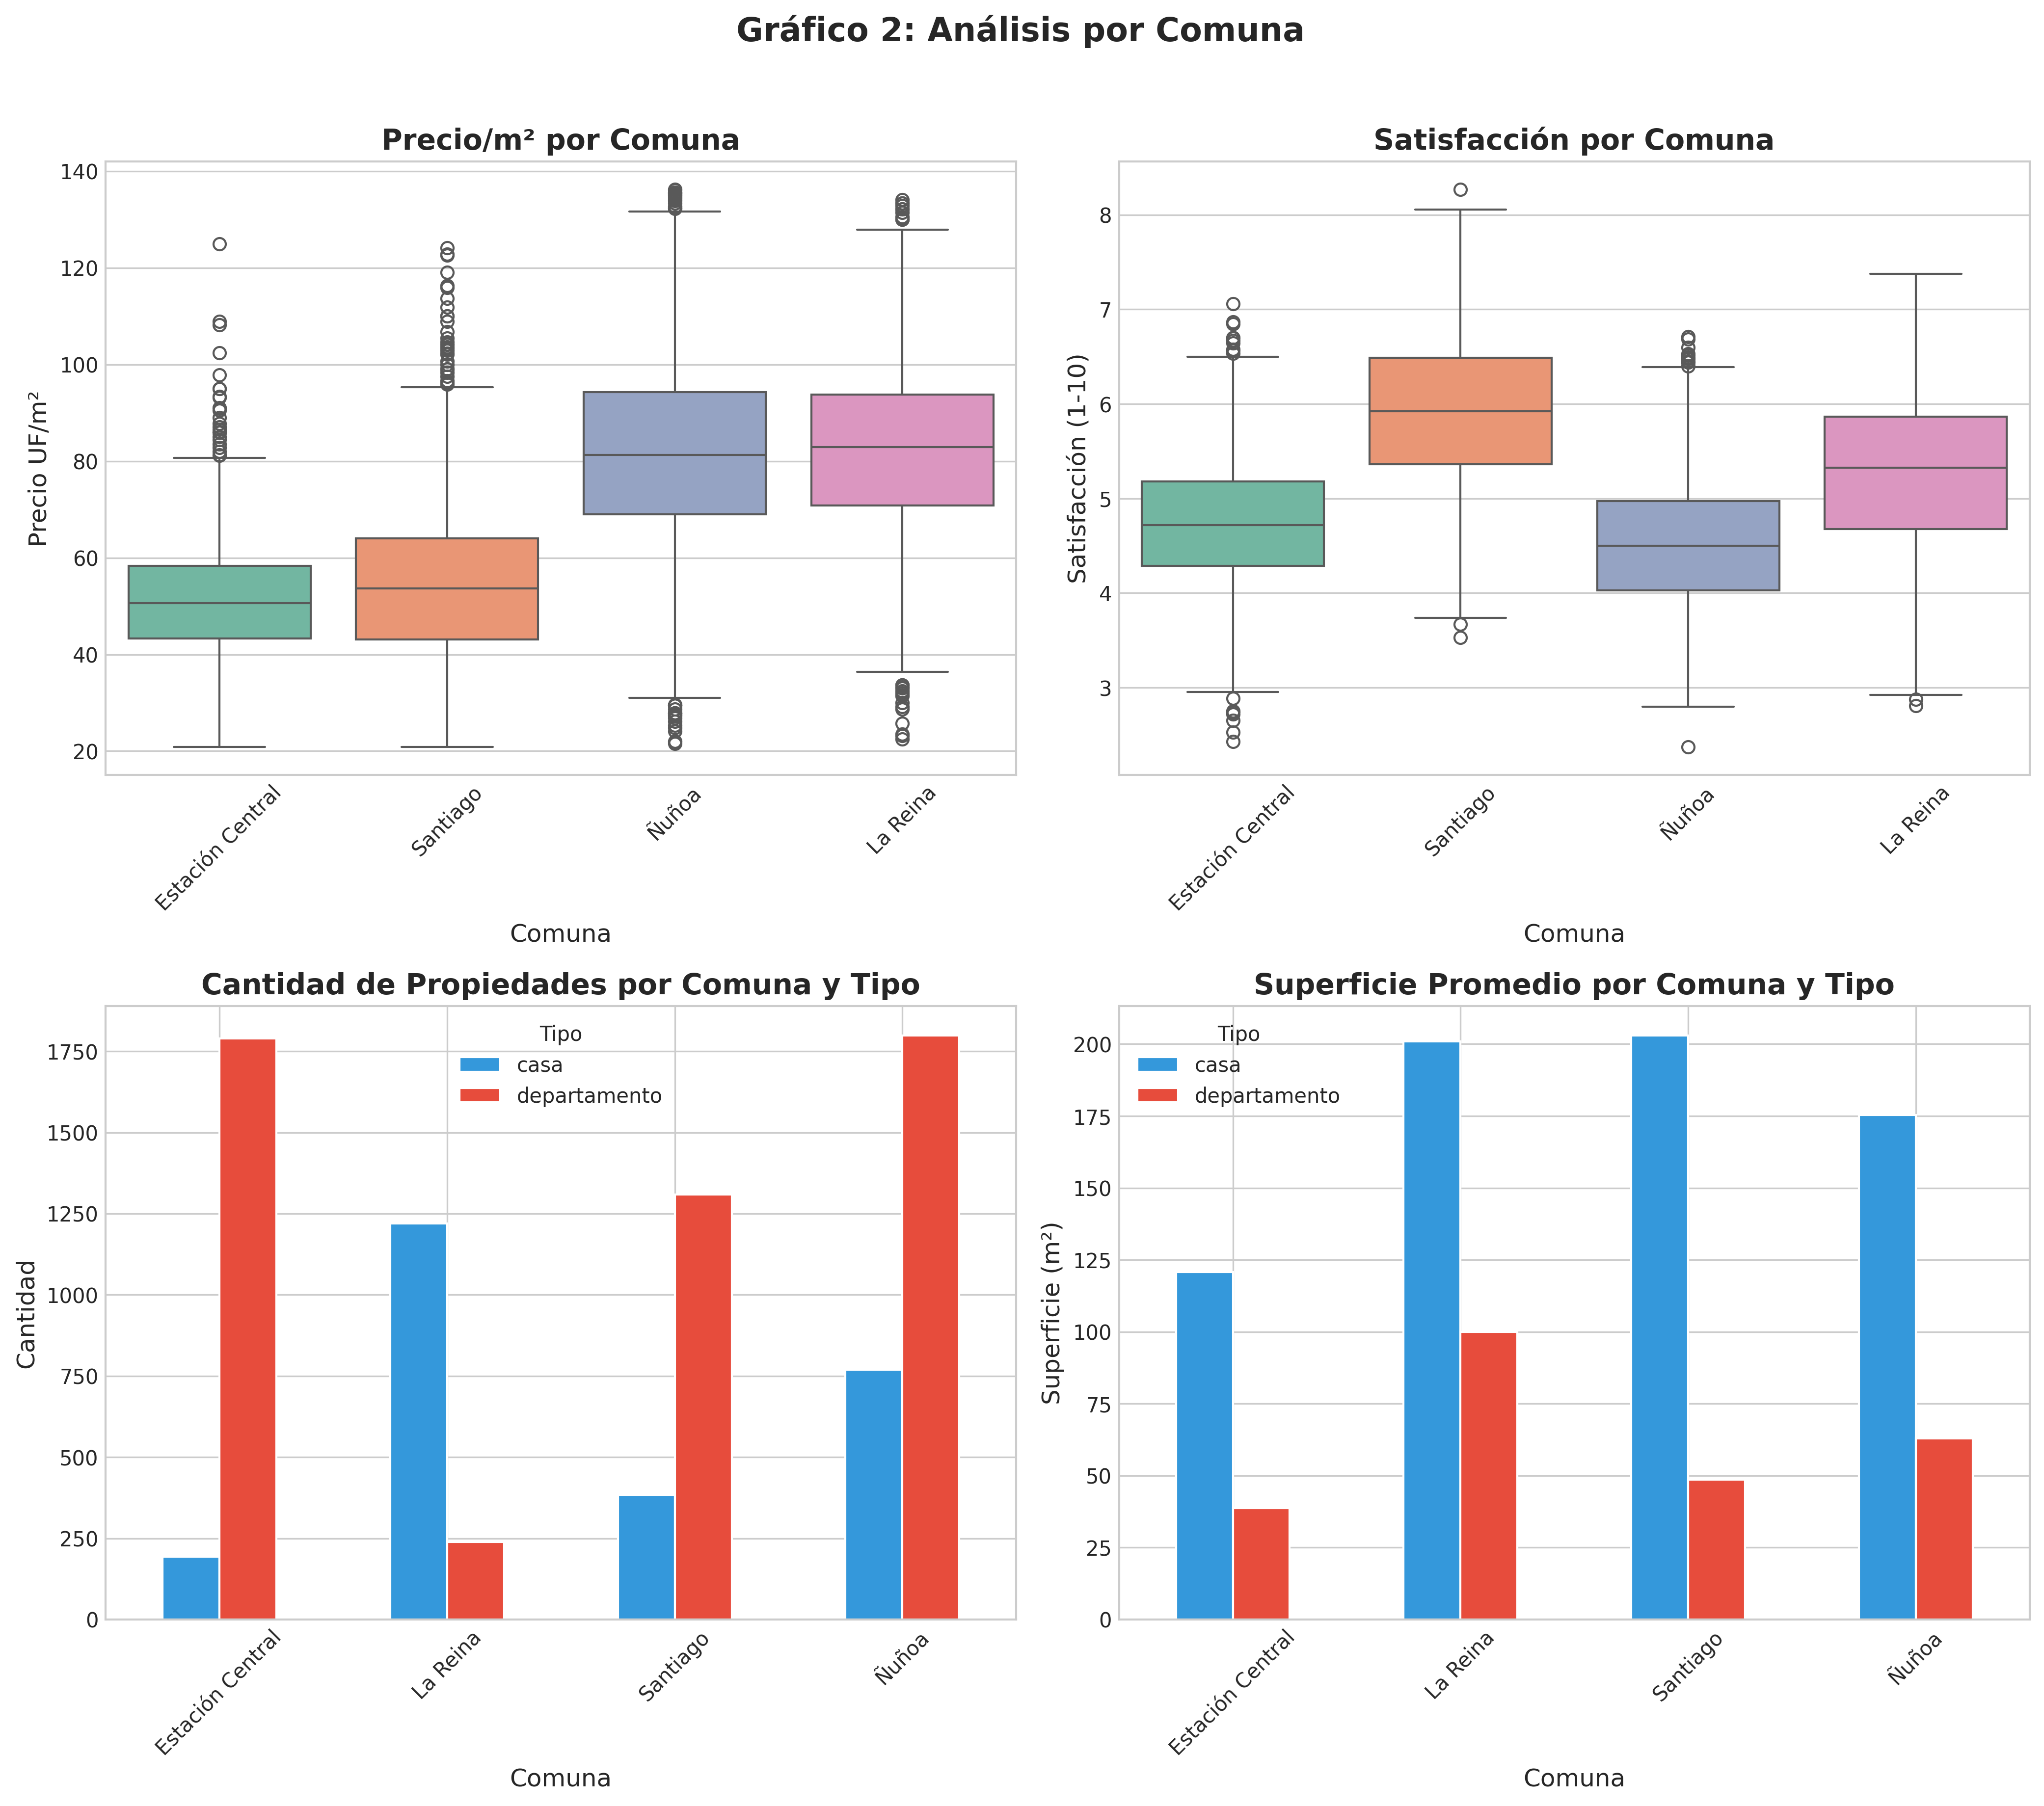
\includegraphics[width=0.95\textwidth]{figuras/grafico_02_analisis_comunas.png}
    \caption{Análisis comparativo de propiedades por comuna: distribución de precios, superficies y características}
    \label{fig:analisis_comunas}
\end{figure}

\begin{figure}[H]
    \centering
    % 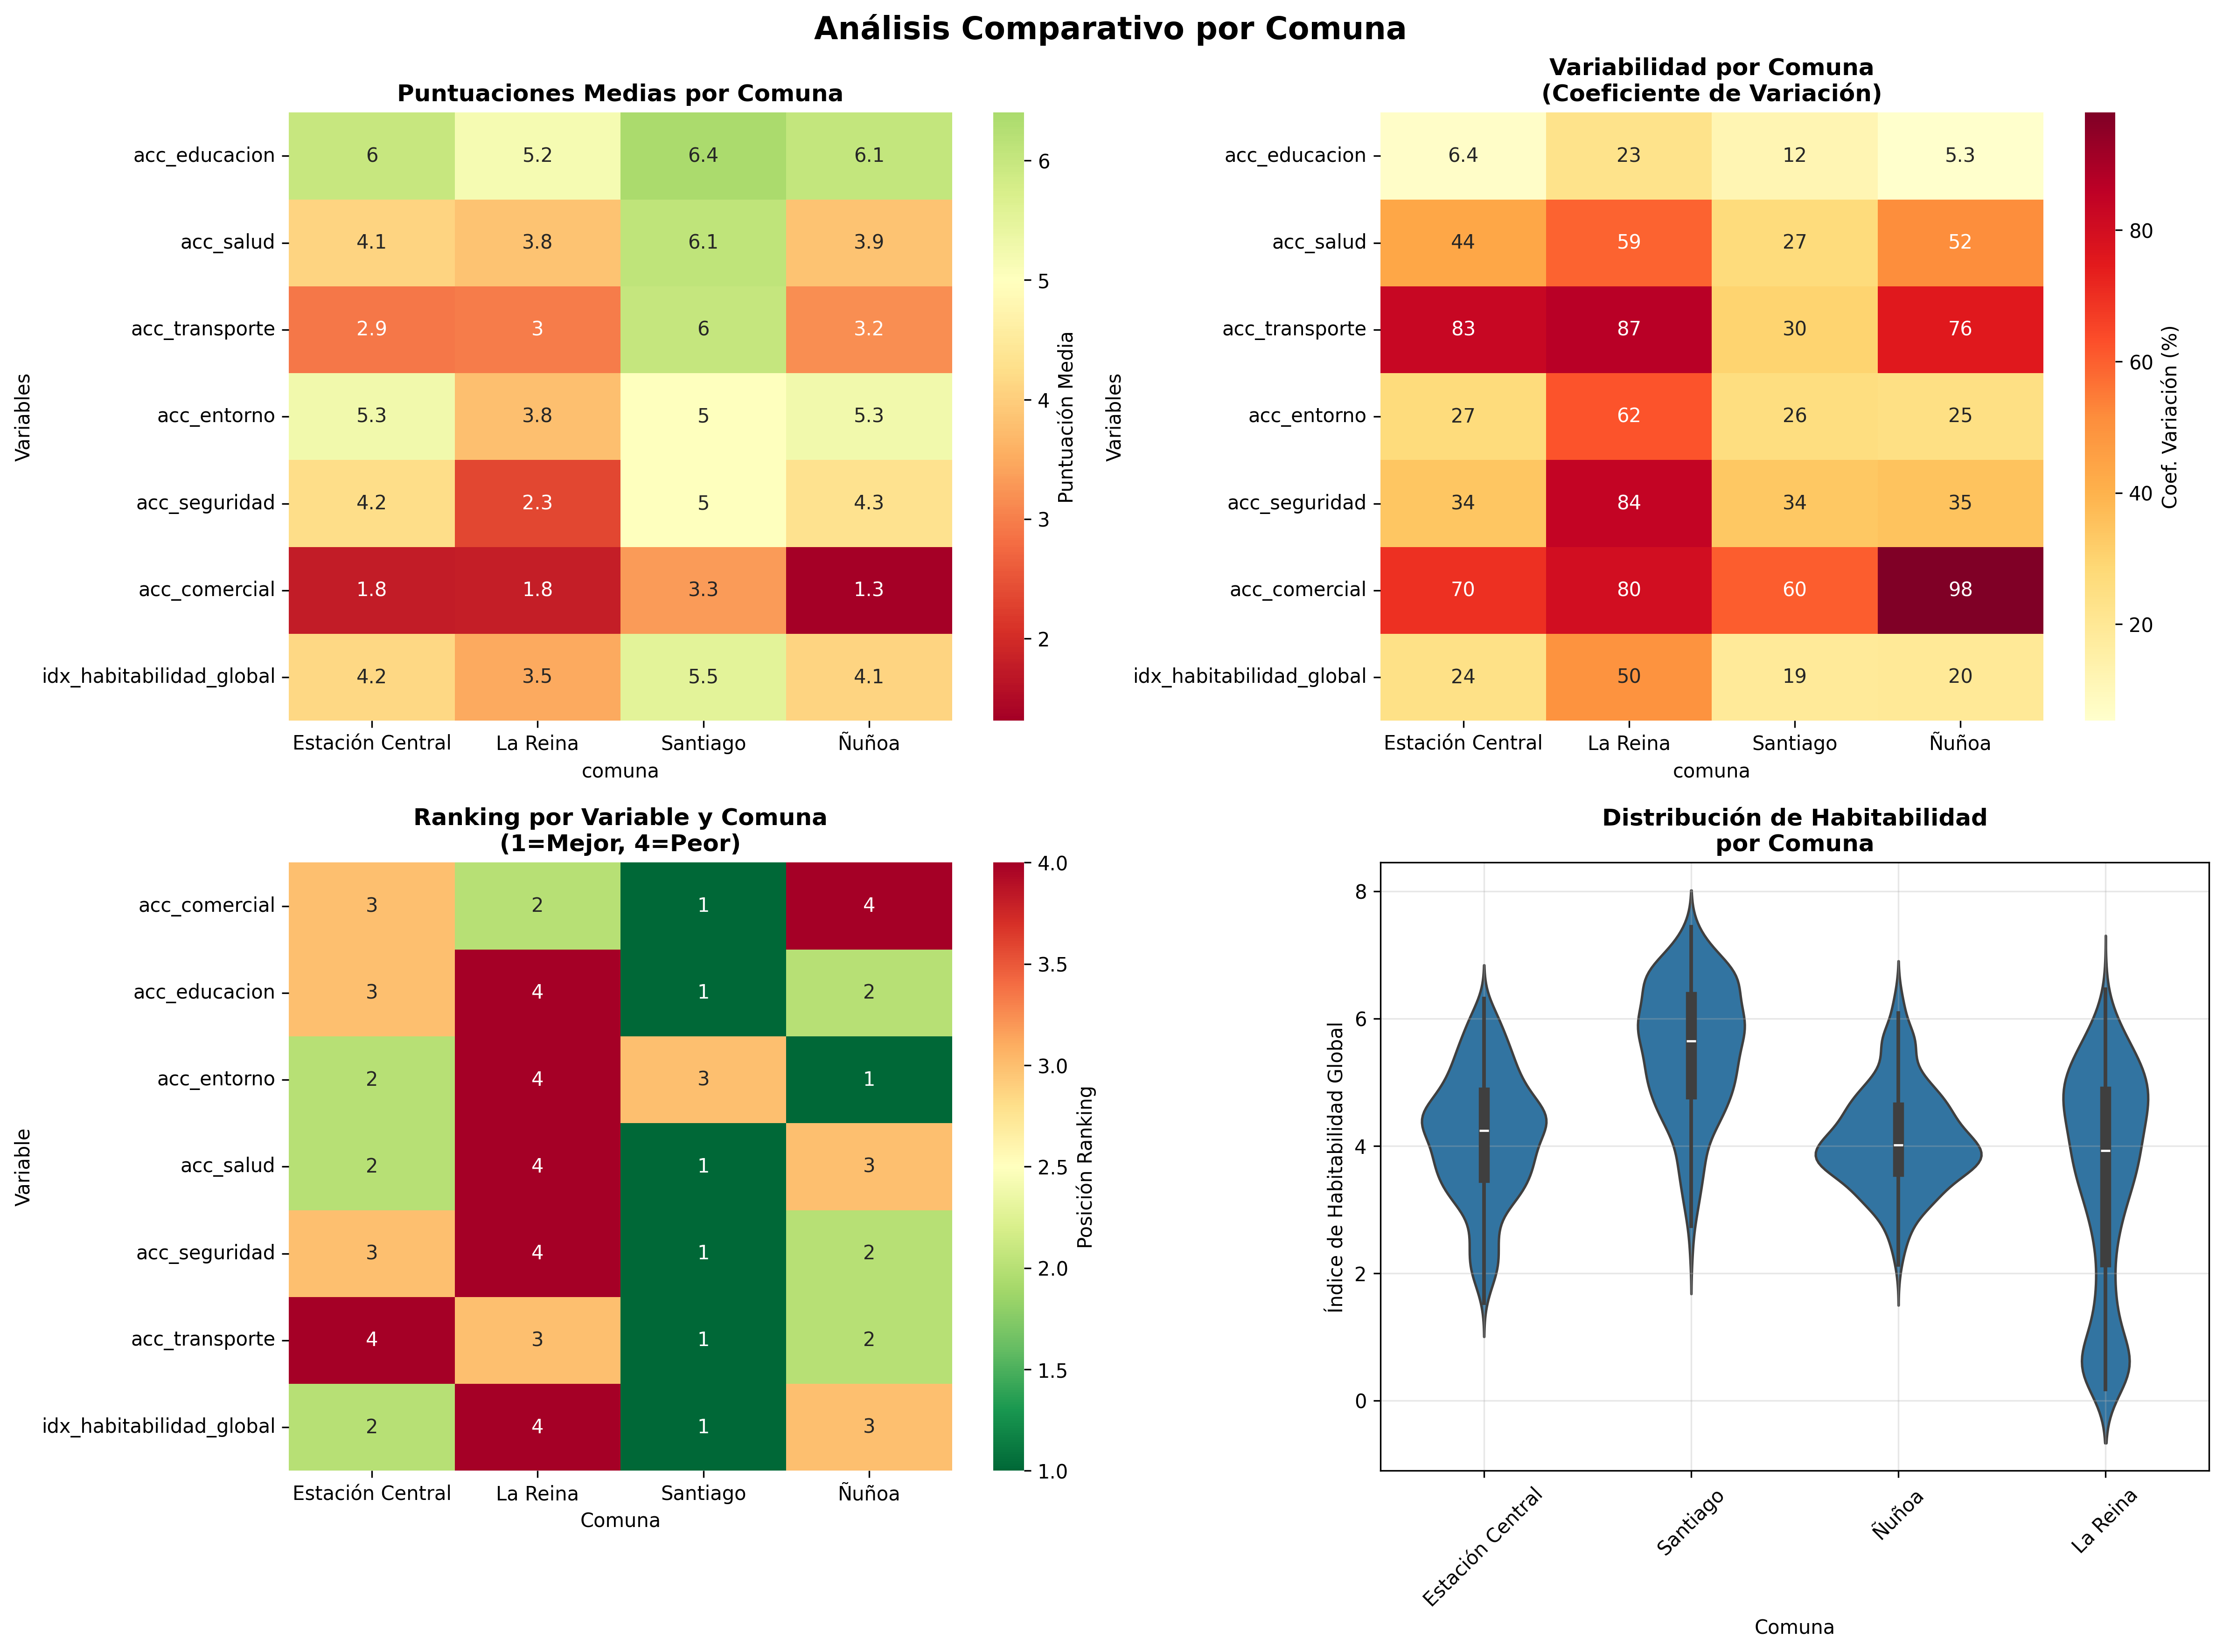
\includegraphics[width=0.9\textwidth]{figuras/10_analisis_por_comuna.png}
    \caption{Análisis detallado de características espaciales por comuna}
    \label{fig:detalle_comunas}
\end{figure}

\subsubsection{Distribuciones Espaciales}

\begin{figure}[H]
    \centering
    % 
\includegraphics[width=0.9\textwidth]{figuras/mapa_02_precio_m2.png}
    \caption{Distribución espacial del precio por metro cuadrado (UF/m²) en las 4 comunas}
    \label{fig:mapa_precios}
\end{figure}

\begin{figure}[H]
    \centering
    
\includegraphics[width=0.9\textwidth]{figuras/mapa_03_satisfaccion_predicha.png}
    \caption{Mapa de satisfacción residencial predicha por el modelo LightGBM}
    \label{fig:mapa_satisfaccion}
\end{figure}



\subsubsection{Relación Predicción vs. Realidad}

\begin{figure}[H]
    \centering
    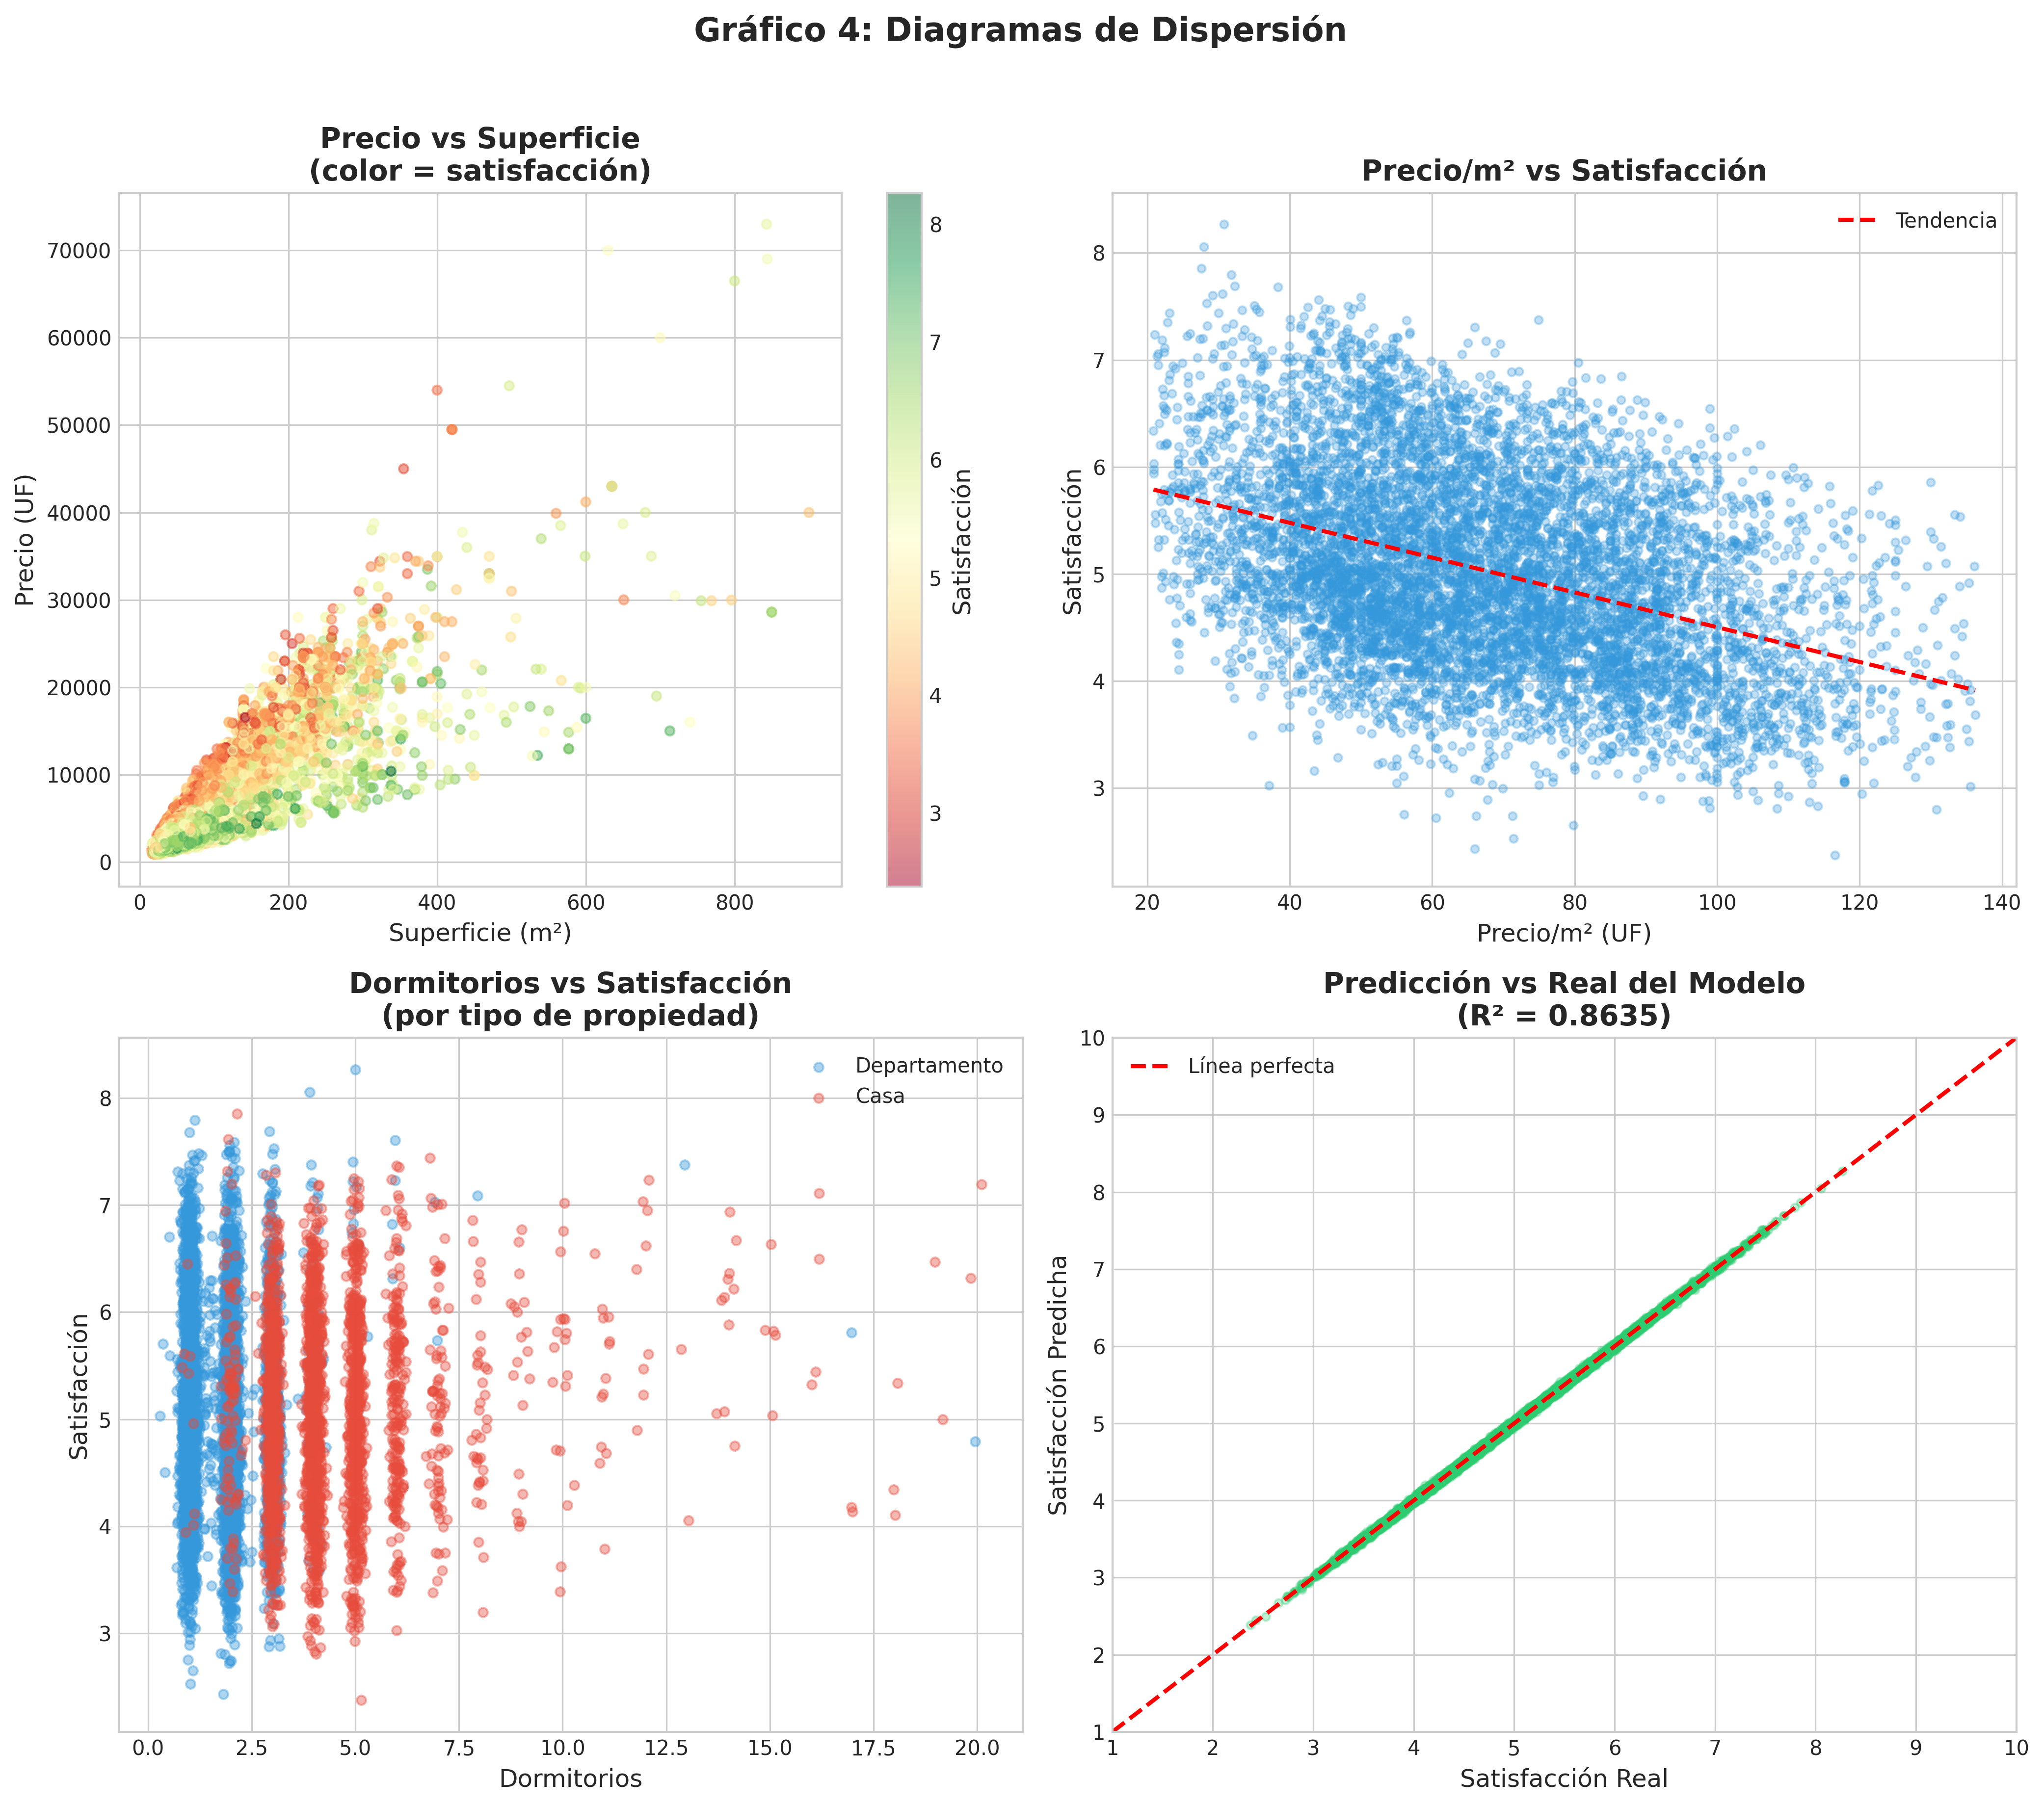
\includegraphics[width=0.8\textwidth]{figuras/grafico_04_dispersion.png}
    \caption{Gráfico de dispersión: satisfacción predicha vs. satisfacción real (R² = 0.8635)}
    \label{fig:dispersion}
\end{figure}

El gráfico de dispersión (Figura \ref{fig:dispersion}) muestra la relación lineal entre valores predichos y reales, con puntos concentrados cerca de la línea de identidad y=x, confirmando la precisión del modelo LightGBM.

\subsubsection{Importancia de Variables}

\begin{figure}[H]
    \centering
    
\includegraphics[width=0.9\textwidth]{figuras/grafico_05_importancia_metricas.png}
    \caption{Importancia de las 20 principales variables en el modelo predictivo LightGBM}
    \label{fig:importancia}
\end{figure}

La figura \ref{fig:importancia} presenta el ranking de importancia relativa de características, evidenciando el predominio de variables económicas (precio/m²) seguido por características espaciales (distancias a servicios) y atributos físicos de la propiedad.

\subsection{Visualizaciones Interactivas}

El proyecto generó un mapa interactivo HTML utilizando la biblioteca Folium, que permite:

\begin{itemize}
    \item \textbf{Exploración geográfica:} Navegación por las 7,702 propiedades con zoom y pan
    \item \textbf{Información detallada:} Pop-ups con características de cada propiedad
    \item \textbf{Codificación por color:} Visualización de satisfacción predicha mediante escala cromática
    \item \textbf{Capas superpuestas:} Servicios urbanos (educación, salud, transporte) como marcadores
\end{itemize}

Este mapa interactivo se encuentra disponible en el archivo \texttt{mapa\_interactivo.html} y constituye una herramienta de exploración complementaria para usuarios finales del sistema TerraMatch.

\begin{figure}[H]
    \centering
    
\includegraphics[width=0.9\textwidth]{figuras/mapa_03_satisfaccion_predicha.png}
    \caption{Mapa de satisfacción residencial predicha: visualización estática de la distribución espacial de predicciones del modelo LightGBM en las 4 comunas}
    \label{fig:mapa_satisfaccion}
\end{figure}

% Descripción y link a visualizaciones web si existen

% ====================================================================
% 6. IMPLEMENTACIÓN TÉCNICA
% ====================================================================

% ====================================================================
% 7. DISCUSIÓN
% ====================================================================

